\section{Architecture logicielle}
	\label{section:archi}



L'étude du logiciel ADTool a mis en évidence des limitations en ce qui concerne l'analyse d'arbre. Afin d'y remédier de nouvelles fonctionnalités seront implémentées. Ces fonctionnalités se décomposent en deux parties : celles-qui apportent une véritable plus-value pour l'analyse d'arbre, et celles qui facilitent le travail d'édition d'arbre. 

Le projet aboutira donc sur la création d'un nouveau logiciel nommé \glasir{} qui contiendras les nouvelles fonctionnalités d'analyse. Ce logiciel encapsulera une version amélioré d'ADTool qui sera son éditeur d'ADTree. Deux raisons ont motivées la décision de créer un nouveau logiciel. Tout d'abords, cela permet de séparer l'analyse et l'édition des ADTrees, afin d'avoir des logiciels dédiés à leur tâche. Deuxièmement, cette solution permet d'utiliser des technologies différentes de celles d'ADTool, enrichissant ainsi notre formation. La {\sc Figure} \ref{fig:architecture_Glasir} montre l'intégration d'ADTool dans l'architecture de \glasir{}.

	\begin{figure}[h!]
		\centering
			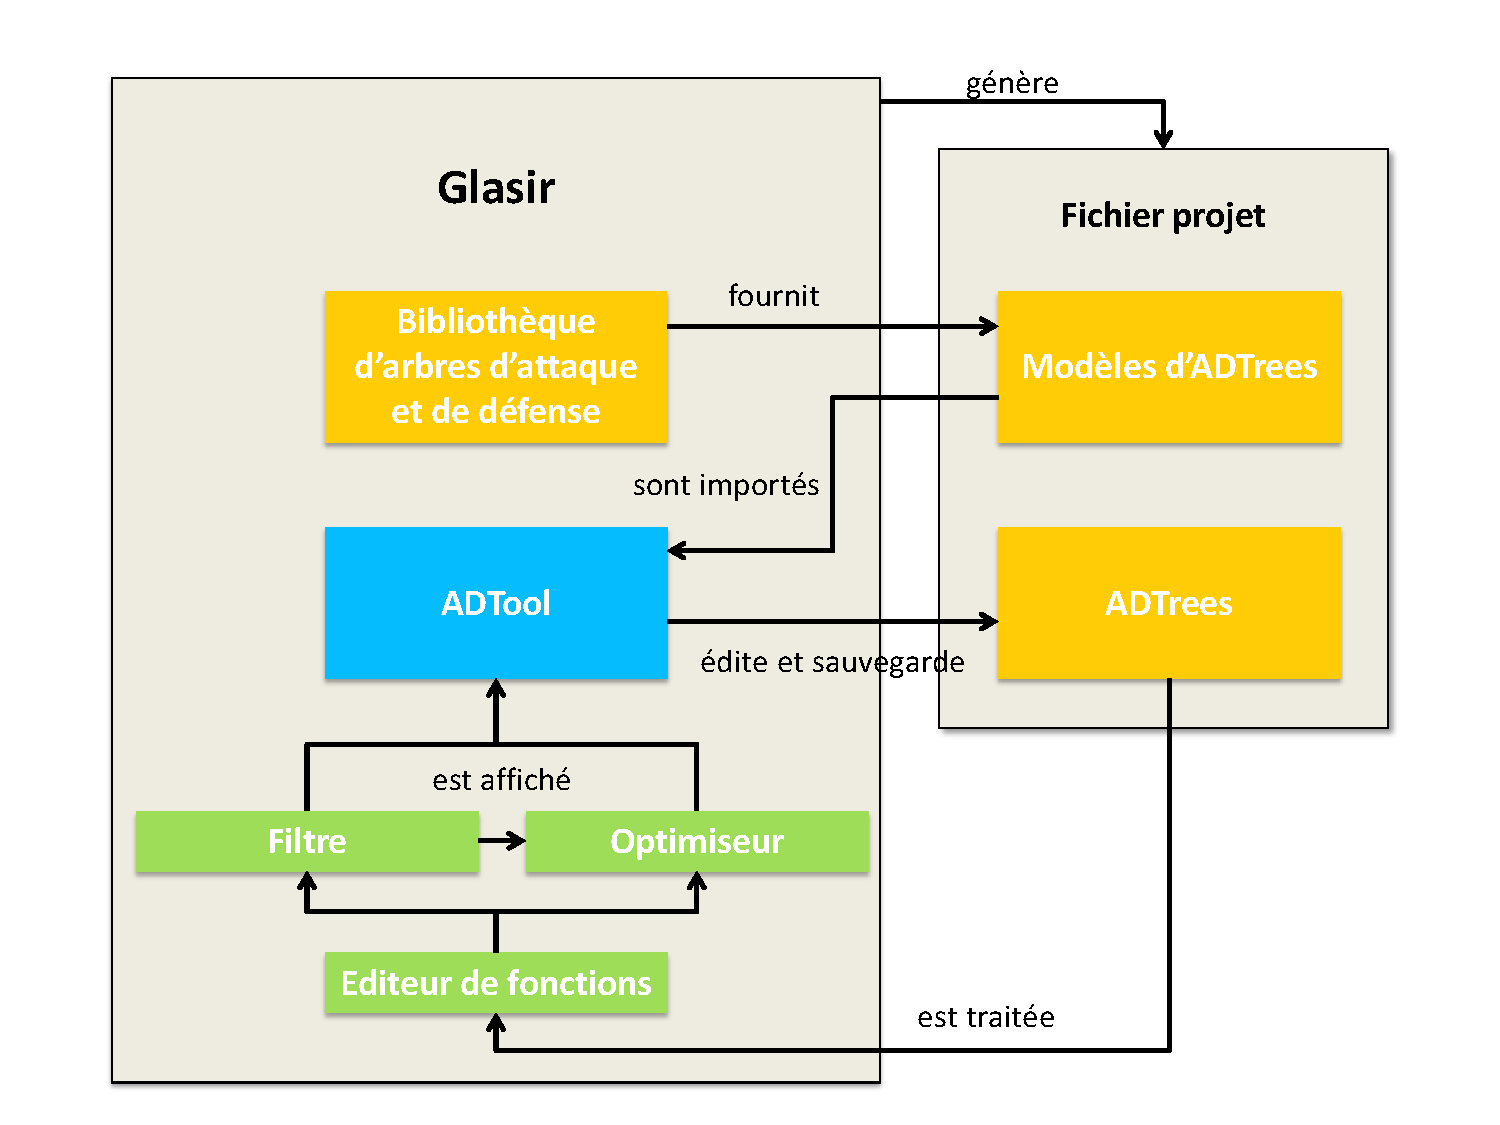
\includegraphics[width=0.8\textwidth]{figure/archiGlasir.pdf}
		\caption{Architecture du logiciel \glasir{}.}
		\label{fig:architecture_Glasir}
	\end{figure}

Comme illustré sur la {\sc Figure} \ref{fig:architecture_Glasir}, \glasir{} est constitué d'une bibliothèque d'ADTrees, d'ADTool et des nouvelles fonctionnalités d'analyse. L'expert réalisant un projet d'analyse à l'aide de \glasir{} utilisera des fichiers projets. Ils contiennent les ADTrees du projet en cours ainsi que les modèles génériques d'ADTrees que l'expert a jugé utiles pour son projet. Ceux-ci proviennent de la bibliothèque d'ADTrees de \glasir{}.
	
Lors de la création d'un projet quelconque, \glasir{} commence par créer le fichier projet correspondant. L'expert va alors créer ou importer ses ADTrees grâce à ADTool. Les modèles de la bibliothèque d'ADTrees utilisés dans le cadre du projet seront également sauvegardés dans le fichier projet, pour gérer leurs éventuelles modifications sans impacter la bibliothèque d'arbres de \glasir{}. L'expert pourra alors définir ses paramètres de synthèse avec l'éditeur de fonction, filtrer grâce au module Filtre ou encore chercher le chemin optimal à l'aide de l'Optimiseur. La prochaine section détaillera l'implémentation de ces modules. 